\section{Arquitectura del backend}

En esta sección se expone cómo está estructurado el servidor del proyecto, los flujos lógicos que sigue, varios puntos interesantes sobre su funcionamiento, y las diferentes rutas con las que cuenta la API.

\subsection{Estructura del backend}
El servidor se organiza en módulos interconectados para ofrecer servicios robustos al frontend y facilitar un desarrollo escalable.
Una petición HTTP sigue esta secuencia: el cliente consume una ruta (endpoint), se ejecutan los middlewares de autenticación y/o carga de imágenes si corresponde, y un controlador procesa los datos interactuando con uno o varios modelos para luego devolver la respuesta que corresponda. Por ello, se distinguen los siguientes modulos principales:

\begin{itemize}
    \item \textbf{Entrada y Configuración Inicial}: En la raíz del proyecto se encuentra el archivo \texttt{index.js}, encargado de configurar y levantar el servidor. Para ello, se conecta a la base de datos y carga los endpoints y los middlewares pertinentes.

    Para que el frontend tenga acceso a la API, es esencial configurar el mecanismo de seguridad \textbf{CORS (Cross-Origin Resource Sharing)}. En una arquitectura desacoplada como la de este proyecto, el cliente y el servidor suelen operar en dominios o puertos distintos. Por seguridad, los navegadores modernos aplican la "Política de Mismo Origen" (\textit{Same-Origin Policy}), que prohíbe que un script cargado en un origen acceda a recursos de otro distinto. Con la configuración de \texttt{CORS} se define una lista de dominios autorizados a acceder a la API, así como habilitar el intercambio de credenciales.

    \begin{figure}[h]
    \centering
    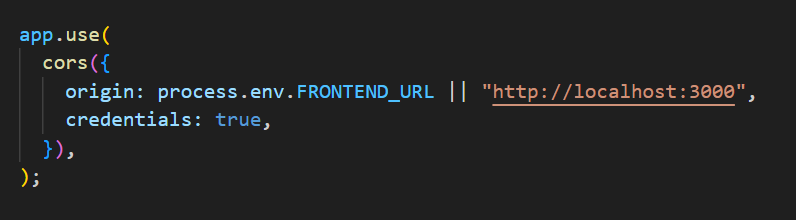
\includegraphics[width=0.8\textwidth]{imagenes/cors.png}
    \caption{Configuración del CORS en la entrada del backend}
    \label{fig:cors}
    \end{figure}

    \item \textbf{Lógica de negocio}: la lógica de negocio se organiza en una estructura con tres partes, basándose en el principio de separación por responsabilidades ("SoC" o Separation of Concerns), que busca dividir sistemas complejos en partes más pequeñas y manejables cada una de las cuales cubre una funcionalidad. Así, tenemos la definición de los puntos de acceso (\texttt{routes/}), la implementación de las reglas de negocio (\texttt{controllers/}) y la definición de los modelos de datos (\texttt{models/}).

    \item \textbf{Middlewares}: La carpeta (\texttt{middlewares/}) incluye las configuraciones de autenticación de usuario y de subida de archivos, que se explicarán en detalle más adelante.
\end{itemize}

Además, el proyecto cuenta con la carpeta \texttt{templates/}, que contiene la plantilla para enviar correos automatizados; y la carpeta \texttt{uploads/profile\_pictures/}, que actúa como almacenamiento local para las imágenes de perfil de los usuarios.


Esta separación garantiza que el sistema sea escalable y fácil de mantener.


\subsection{Emails automatizados}
La función del backend encargada la generación de códigos de verificación y su envío via email al usuario, que se emplea tanto para el registro de una nueva cuenta como para la recuperación de sus credenciales en caso de olvido; es capaz de realizar sus tareas de forma automatizada gracias a un transportador que utiliza el servicio SMTP (Simple Mail Transfer Protocol, un protocolo de red para intercambiar mensajes de correo electrónico) de Gmail. Un transportador es un objeto de configuración donde se define este servicio SMTP y se inyectan las credenciales para utilizarlo, es decir, la cuenta de correo electrónico y su contraseña.

En realidad, ya no se utiliza la contraseña de la cuenta de correo directamente, Google bloqueó eso por ser una práctica poco segura y la sustituyó por Google App Password, códigos de 16 caracteres que se pueden obtener en la configuración de la cuenta de Google y que actúan como las credenciales para usar nuestra cuenta de correo de Gmail mediante código. Estas credenciales se pueden obtener solamente al tener la 2FA (2 Factor Authentication) de Google activada, y se pueden revocar de una aplicación u otra cuando se necesite; manteniendo así las credenciales primarias seguras.

Lo que se envía en estos correos automatizados es una plantilla HTML con el código de verificación generado. De esta forma, el email que reciben los usuarios es visualmente agradable y fácil de entender en un vistazo. Así es como se ve:

\begin{figure}[H]
    \centering
    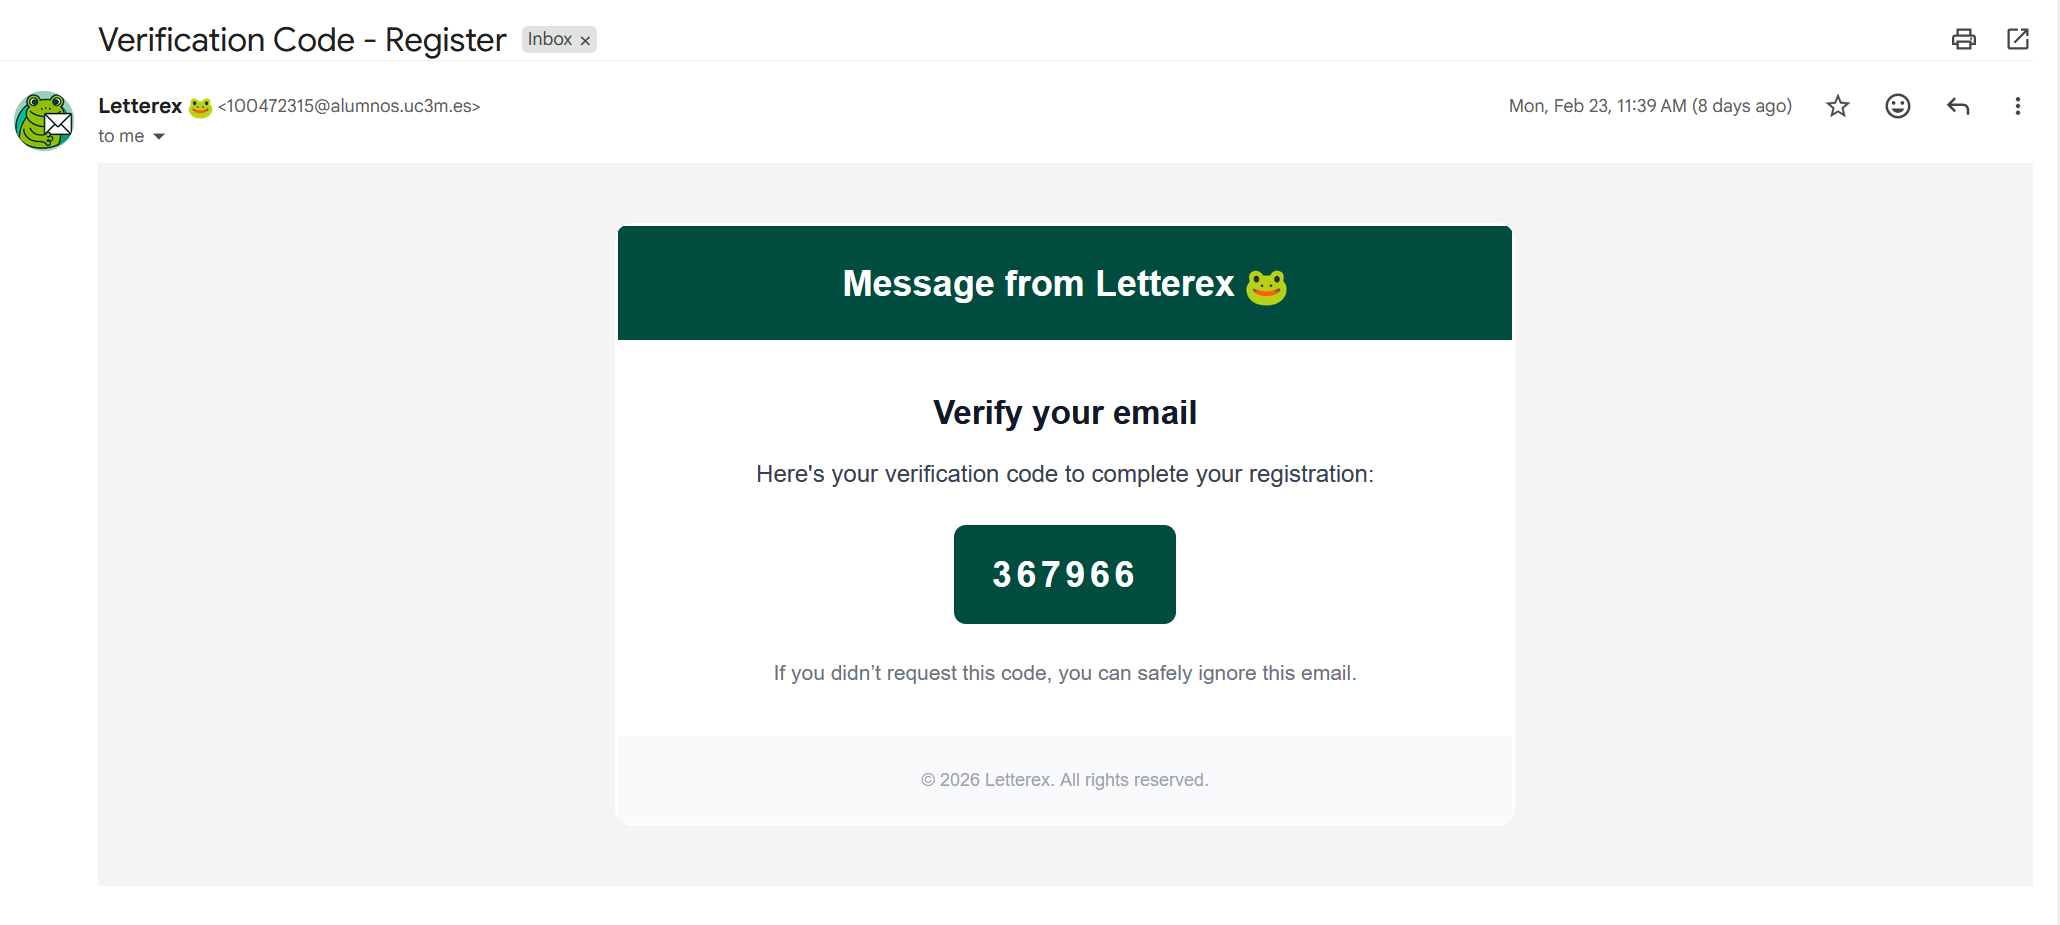
\includegraphics[width=\textwidth]{./imagenes/template_email.png}
    \caption{Email automatizado}
    \label{fig:email}
\end{figure}

\subsection{Mecanismo de Autenticación y Autorización}
Al acceder a la plataforma introduciendo su nombre de usuario o email y contraseña, el usuario recibe un token que contiene información de la sesión como el momento en que inició, el momento de caducidad, y los datos no sensibles del usuario. Se trata de un token JWT (JSON Web Token) \cite{jwtio}, un contenedor de información seguro y compacto que permite verificar la identidad del cliente en cada interacción con la API.

\begin{figure}[H]
    \centering
    
\includegraphics[height=3cm]{./imagenes/jwt.png}
    \caption{JSON Web Tokens}
    \label{fig:jwt}
\end{figure}

Este token se envia desde el backend y se almacena en el navegador mediante \textit{cookies}, con el objetivo de que el navegador pueda recordar la sesión del usuario. Al cerrar la sesión, esta cookie se elimina. El navegador adjunta automáticamente el token a las solicitudes HTTP que envía al servidor. De esta forma, el servidor es capaz de identificar al usuario y aplicar los permisos correspondientes sin necesidad de consultar una tabla de sesiones activa en la base de datos, lo que optimiza los recursos del sistema.

Sobre el refuerzo de la seguridad de la cookie, hay dos puntos interesantes que mencionar. En primer lugar, la cookie es HttpOnly, es decir, no se puede leer mediante JavaScript sino que solo puede leerla el navegador. De esta forma, el token está protegido contra ataques maliciosos como \textbf{Cross-Site Scripting (XSS)}, una vulnerabilidad en la que un atacante inyecta y ejecuta código malicioso (generalmente de JavaScript) en el navegador de otros usuarios que usan la aplicación.

En segundo lugar, se ha implementado el atributo \textbf{SameSite} con el valor \texttt{"Strict"}. Esta configuración es una medida de seguridad crítica para prevenir ataques de tipo \textbf{CSRF (Cross-Site Request Forgery)}, que aprovechan la naturaleza automática de los navegadores, dado que estos adjuntan las cookies de sesión a cualquier petición dirigida al dominio de origen. El atacante podría engañar a un usuario autenticado para que haga clic en un enlace malicioso en una pestaña diferente, y dicho enlace dispararía una petición a nuestra API (por ejemplo, para borrar una carta o cambiar la contraseña). Con la configuración de SameSite, este tipo de ataques son mitigados.

Al llegar una solicitud HTTP al sistema, si se trata de una ruta protegida se ejecuta el \textbf{Middleware de Autenticación}. Este componente intercepta la solicitud, extrae el token JWT de la cookie y verifica su validez. Si es válido, el middleware decodifica la información del usuario y la inyecta en el objeto de la petición, permitiendo que el resto del flujo identifique al autor de la acción, es decir, el usuario autenticado en la aplicación.

Estas decisiones técnicas refuerzan la robustez del sistema y aseguran que cada acción realizada en este sea legítima y provenga exclusivamente de la interacción directa del usuario con la interfaz oficial, de forma que usuario pueda acceder de forma segura a las acciones que requieren su autenticación.

\subsection{Almacenamiento de imágenes con Multer y Cloudinary}

Para la gestión de imágenes de perfil, se ha implementado una solución que combina la librería \textbf{Multer} para el procesamiento eficiente de archivos con \textbf{Cloudinary} como servicio de almacenamiento en la nube. Multer es una librería que facilita la subida de archivos mediante formularios web para aplicaciones de Node.js. Por su parte, Cloudinary es un servicio de gestión de recursos digitales, en especial imágenes y vídeos, que proporciona almacenamiento persistente en la nube y optimización automática. \cite{llamas_multer_nd, cloudinary_official_2026,moge_cloudinary_2026}

La configuración del sistema de subida de archivos se divide en tres pilares fundamentales:

\begin{itemize}
    \item Procesamiento en memoria: Se utiliza Multer para interceptar y procesar la subida de archivos directamente en memoria con un búfer, evitando la necesidad de almacenamiento temporal en disco. Una decisión de diseño clave ha sido el renombrado del archivo por el identificador del usuario extraído del token de autenticación, de modo que cada usuario posea una única imagen de perfil en Cloudinary. En caso de actualización, se sobrescribe la imagen anterior automáticamente, eliminando la necesidad de gestionar manualmente archivos obsoletos.

    \item Almacenamiento en la nube: Una vez procesado el búfer, la imagen se sube directamente a Cloudinary. El sistema almacena la URL segura retornada por Cloudinary en la base de datos, facilitando un acceso rápido sin depender del almacenamiento local del servidor. Además, Cloudinary aplica transformaciones automáticas, como la limitación de dimensiones a 800x800 píxeles, para garantizar consistencia visual y reducir consumo de ancho de banda.
    \item Filtrado de seguridad: Para prevenir la subida de archivos maliciosos (como \textit{scripts} ejecutables disfrazados), se ha implementado un filtro por tipo MIME y extensión. El sistema solo acepta formatos de imagen estándar (\texttt{JPEG, JPG, PNG}), verificando tanto la extensión del archivo como su tipo MIME real para asegurar la integridad del recurso. También, se establece un máximo de tamaño del archivo de 5 MB para evitar \textbf{ataques de denegación de servicio (DoS)} por agotamiento de almacenamiento o ancho de banda.

\end{itemize}

Este módulo se exporta como un middleware independiente, lo que permite inyectarlo exclusivamente en las rutas de la API que requieren capacidad de subida, manteniendo así el principio de responsabilidad única en el código. Además, la integración con Cloudinary elimina la dependencia de la infraestructura local de almacenamiento, proporcionando escalabilidad y disponibilidad.

\subsection{Interfaz de Programación de Aplicaciones (API): Rutas y Controladores}

El backend de la plataforma actúa como una capa de servicios diseñada para que el frontend interactúe con la base de datos de forma segura y eficiente. Esta comunicación se articula mediante una \textbf{API RESTful}, que expone una serie de puntos de entrada o endpoints organizados por recursos (usuarios, cartas, correcciones, etc.).

La lógica de interacción se fundamenta en las operaciones \textbf{CRUD} (\textit{Create, Read, Update, Delete}), que representan las acciones esenciales para la gestión de persistencia de datos. En este proyecto, dichas acciones se mapean directamente con los métodos del protocolo \textbf{HTTP}, garantizando una arquitectura estandarizada:

\begin{itemize}
    \item \textbf{POST (Create)}: Utilizado para la creación de nuevos documentos, como el registro de un usuario o el envío de una nueva carta.
    \item \textbf{GET (Read)}: Empleado para la recuperación de información, ya sea una lista de recursos o un documento específico identificado por su ID.
    \item \textbf{PUT / PATCH (Update)}: Destinados a la actualización de registros existentes. Se utiliza \texttt{PUT} para sustituciones integrales y \texttt{PATCH} para modificaciones parciales, como marcar una carta como "leída".
    \item \textbf{DELETE (Delete)}: Encargado de la eliminación de recursos o, en el caso de las cartas, de la activación del borrado lógico mencionado anteriormente.
\end{itemize}

Cada ruta definida en el servidor está vinculada a un \textbf{controlador} específico, el cual contiene la lógica final para procesar la solicitud. Una vez superada la fase de autenticación, la ejecución pasa al controlador específico correspondiente, cuya función es extraer los parámetros de la consulta, utilizar la identidad del usuario ya validada para aplicar reglas de negocio, ejecutar las operaciones correspondientes en MongoDB mediante los modelos de Mongoose, y devolver una respuesta HTTP con los datos en formato JSON y un código de éxito o error.

A continuación, se muestra una tabla con todos los métodos que se han desarrollado para esta API y de los que el frontend más adelante se servirá. Estás separados en categorías según el controlador y enrutador que se encarga de ellos: User, Letter, CorrectedLetter y Follow. Podría crearse uno nuevo para los modelos de VerificationCode y FriendRequest, pero por simplicidad se han incluido las pocas funciones de estos en el grupo de User y Follow, respectivamente. Además, se marca con un asterisco los valores de entrada obligatorios.

\begin{longtable}{|l|p{5cm}|p{8cm}|}
\hline
\textbf{Función} & \textbf{Ruta} & \textbf{Descripción} \\
\hline
\endhead
\hline
\endfoot
\multicolumn{3}{|c|}{\textbf{User Routes}} \\
\hline
POST & /api/users/register & Registrar un nuevo usuario. \newline \textbf{Valores de entrada:} nickname*, email*, password*, master\-Language*, learning\-Language* \newline \textbf{Valores de salida:} status, message, user \\
POST & /api/users/login & Iniciar sesión. Si las credenciales recibidas son correctas, se crea y envía la cookie de autenticación. \newline \textbf{Valores de entrada:} email* (string, puede ser email o nickname), password* \newline \textbf{Valores de salida:} status, userData, token, cookie authToken \\
POST & /api/users/logout & Cerrar la sesión. Se limpia la cookie de autenticación. \newline \textbf{Valores de entrada:} ninguno \newline \textbf{Valores de salida:} status, message \\
GET & /api/users/profile/:id? & Obtener los datos del perfil de usuario cuyo id es especificado en la ruta, o en su defecto (es un parámetro opcional, de ahí el signo de interrogación en la ruta) del usuario autenticado.\newline \textbf{Valores de salida:} status, user \\
GET & /api/users/list-users/:page? & Listar usuarios con paginación. Si no se recibe el parámetro page, que indica la página que se pide, se entregan los usuarios de la primera página. \newline \textbf{Valores de salida:} status, users, page, itemsPerPage, totalUsers, totalPages \\
PUT & /api/users/update & Actualizar datos del usuario autenticado. \newline \textbf{Valores de salida:} status, userData \\
PUT & /api/users/change-password & Cambiar contraseña actual. \newline \textbf{Valores de salida:} status, message \\
PUT & /api/users/profile-picture & Subir foto de perfil. Se trata de un método PUT porque no solo sube una nueva imagen al sistema de archivos sino que modifica los datos del usuario.\newline \textbf{Valores de salida:} status, userId, profilePicture \\
DELETE & /api/users/profile-picture & Eliminar foto de perfil. \newline \textbf{Valores de salida:} status, message \\
GET & /api/users/profile-picture/:id & Obtener foto de perfil de un usuario. En caso de que el parámetetro id no esté especificado, se entrega la del usuario autenticado. \newline \textbf{Valores de salida:} Archivo (imagen) \\
GET & /api/users/check-nickname/:nickname & Verificar disponibilidad de nickname. \newline \textbf{Valores de salida:} status, inUse: boolean \\
GET & /api/users/check-email/:email & Verificar si email está registrado. \newline \textbf{Valores de salida:} result, inUse: boolean \\
POST & /api/users/verification-code & Enviar código de verificación. \newline \textbf{Valores de entrada:} email*, purpose \newline \textbf{Valores de salida:} message \\
POST & /api/users/check-code & Verificar código de verificación. \newline \textbf{Valores de entrada:} email*, code*, purpose \newline \textbf{Valores de salida:} status, message \\
PUT & /api/users/reset-password & Restablecer contraseña con código de verificación. \newline \textbf{Valores de salida:} status, message \\
DELETE & /api/users/delete-account & Eliminar cuenta de usuario. \newline \textbf{Valores de salida:} status, message \\
\hline
\hline
\multicolumn{3}{|c|}{\textbf{Letter Routes}} \\
\hline
POST & /api/letters/new & Guardar una carta nueva. \newline \textbf{Valores de entrada:} title*, content*, language*, created\_at*, diary \newline \textbf{Valores de salida:} status, message, letter \\
GET & /api/letters/view/:letterId & Obtener información y contenido de una carta.\newline \textbf{Valores de salida:} status, letter, sharedWithDetails \\
PUT & /api/letters/edit/:id & Editar una carta existente. \newline \textbf{Valores de salida:} status, message, letter \\
PUT & /api/letters/edit-diary & Editar el diario de una carta. \newline \textbf{Valores de salida:} status, message, letter \\
DELETE & /api/letters/delete/ & Eliminar una o varias cartas. \newline \textbf{Valores de salida:} status, message \\
GET & /api/letters/list & Listar todas las cartas del usuario. \newline \textbf{Valores de salida:} status, letters, count \\
GET & /api/letters/list/search & Buscar cartas por título. \newline \textbf{Valores de salida:} status, letters \\
POST & /api/letters/share/:id & Compartir una carta con otro usuario (uno o varios). \newline \textbf{Valores de entrada:} shared\-With* \newline \textbf{Valores de salida:} \{message, letter, correctedLetters\} \\
GET & /api/letters/diaries & Listar diarios del usuario. \newline \textbf{Valores de salida:} status, diaries \\
GET & /api/letters/count/:id? & Contar cartas por idioma. Si no se especifica id en la ruta, se cuentan las del usuario autenticado. \newline \textbf{Valores de salida:} Array de \{language, count\} \\
\hline
\hline
\multicolumn{3}{|c|}{\textbf{Follow Routes}} \\
\hline
POST & /api/follow/add/:id & Mandar una solicitud de amistad a un usuario. \newline \textbf{Valores de salida:} status, message \\
DELETE & /api/follow/unfollow/:id & Dejar de seguir a un usuario. \newline \textbf{Valores de salida:} status, message \\
GET & /api/follow/request/:id & Verificar si existe solicitud de amistad. \newline \textbf{Valores de salida:} status, exists: boolean \\
GET & /api/follow/friends & Obtener lista de amigos. \newline \textbf{Valores de salida:} status, count, friends \\
GET & /api/follow/non-friends & Obtener usuarios no agregados. \newline \textbf{Valores de salida:} status, users, totalUsers, totalPages \\
GET & /api/follow/non-friends/:filter & Obtener no usuarios no agregados con un filtro por su nickname. \newline \textbf{Valores de salida:} status, users, totalUsers, totalPages \\
GET & /api/follow/suggested & Obtener usuarios sugeridos. Son usuarios a los que el usuario autenticado no sigue y que tienen idiomas en común con este. \newline \textbf{Valores de salida:} status, suggestedUsers \\
POST & /api/follow/request/:id & Enviar solicitud de amistad. \newline \textbf{Valores de salida:} status, message, friendRequest \\
GET & /api/follow/requests & Listar solicitudes de amistad recibidas. \newline \textbf{Valores de salida:} status, requests \\
POST & /api/follow/accept/:id & Aceptar solicitud de amistad. \newline \textbf{Valores de salida:} status, message \\
POST & /api/follow/decline/:id & Rechazar solicitud de amistad. \newline \textbf{Valores de salida:} status, message \\
\hline
\hline
\multicolumn{3}{|c|}{\textbf{Corrected Letter Routes}} \\
\hline
PATCH & /api/corrected-letters/send-back/:corrected\-Letter\-Id & Mandar de vuelta su autor la carta corregida. \newline \textbf{Valores de salida:} status, message, correctedLetter \\
GET & /api/corrected-letters/corrections/:original\-Letter\-Id & Obtener correcciones de una carta. \newline \textbf{Valores de salida:} status, corrections \\
GET & /api/corrected-letters/corrected\-Letter/:corrected\-Letter\-Id & Obtener corrección específica por ID. \newline \textbf{Valores de salida:} status, correctedLetter \\
GET & /api/corrected-letters/received/ & Obtener cartas recibidas para corregir. \newline \textbf{Valores de salida:} status, correctedLetters, count \\
GET & /api/corrected-letters/received/search & Buscar cartas recibidas por un filtro "search". \newline \textbf{Valores de salida:} status, correctedLetters \\
PUT & /api/corrected-letters/update/:corrected\-Letter\-Id & Actualizar correcciones en proceso. Si la carta ya ha sido enviada de vuelta no se puede realizar esta acción. \newline \textbf{Valores de salida:} status, message, correctedLetter \\
GET & /api/corrected-letters/count/:id? & Contar cartas corregidas por idioma. Si no se especifica el id de usuario en la ruta, se cuentan las del usuario autenticado. \newline \textbf{Valores de salida:} Array de \{language, count\} \\
DELETE & /api/corrected-letters/:corrected\-Letter\-Id & Eliminar carta corregida. \newline \textbf{Valores de salida:} status, message \\
\hline
\caption{Rutas de la API de Letterex}
\label{tab:rutas-api}
\end{longtable}



\subsection{Técnicas de optimización}

\subsubsection{Optimización de búsqueda datos}
La lógica de filtrado se procesa íntegramente en el servidor para garantizar la escalabilidad y mejorar la velocidad de la interfaz liberándola de tareas programacionales. El controlador recibe los términos de búsqueda y ejecuta una consulta optimizada en MongoDB. Esto reduce drásticamente el tamaño de los datos transferidos a través de la red en comparación con un filtrado realizado en el lado del cliente sobre la totalidad de los registros.

Además, para mejorar la usabilidad en la búsqueda y filtrado de cartas, se ha implementado un sistema de comunicación eficiente entre el cliente y el servidor. Donde tenemos una barra de búsqueda, en lugar de realizar peticiones por cada pulsación de tecla, lo que derivaría en un consumo excesivo de recursos y latencia en la red, se ha aplicado la técnica de \textbf{debouncing}. Esta técnica sigue la siguiente lógica:

\begin{itemize}
    \item Control de Eventos: Cuando el usuario escribe en el campo de búsqueda, se inicia un temporizador interno.
    \item Retraso Controlado: Si el usuario sigue escribiendo antes de que transcurran un intervalo definido de tiempo (500ms), el temporizador se reinicia.
    \item Petición Asíncrona: Solo cuando el usuario deja de escribir durante el tiempo estipulado, se dispara la solicitud formal a la API.
\end{itemize}

Así, se logra un consumo y envío de recursos mucho más eficiente.

\subsubsection{Procesamiento Avanzado de Datos: Aggregate de MongoDB}

Otra forma de optimización clave utilizada en el desarrollo del backend es el uso del Aggregate o operaciones de agregación de MongoDB \cite{mongodb_aggregation_2026}. Esta herramienta permite acceder a diferentes colecciones y aplicar filtrados, ordenamientos, uniones, proyecciones y paginación en una única operación atómica. Esto evita el procesar grandes volúmenes de datos en la capa de JavaScript o caer en el problema de las \textbf{N+1 consultas} (realizar múltiples peticiones a la base de datos para completar un solo registro). Así, delegamos la carga de procesamiento al motor de la base de datos, manteniendo tiempos de respuesta bajos y escalables.

\begin{comment}
Un ejemplo real implementado es el flujo de trabajo para la búsqueda de cartas, donde se obtienen también los detalles de los usuarios que han enviado correcciones. El proceso se divide en las siguientes etapas:

    \item \textbf{Pre-filtrado y Paginación}: Primero se selecciona un conjunto reducido de documentos mediante un \texttt{\$match} (autor logueado y carta no eliminada), un \texttt{\$sort} cronológico y las etapas \texttt{\$skip} y \texttt{\$limit} para gestionar la paginación. Realizar esto al inicio asegura que las operaciones posteriores, más costosas, solo se apliquen a los resultados visibles.

    \item \textbf{Resolución de Identidades}: Se aplica un \texttt{\$lookup} (equivalente al \textit{join} de SQL) para unir la colección de cartas con la de usuarios. Esto permite resolver los IDs del array \texttt{sharedWith} y obtener los perfiles reales de los destinatarios.

    \item \textbf{Búsqueda de Correcciones}: Seguidamente, se realiza un segundo cruce con la colección CorrectedLetter. Para cada carta, el sistema busca documentos donde la carta original coincida con la actual y el campo \texttt{sentBack} sea verdadero, agrupando estos resultados en un array interno.

    \item \textbf{Transformación de la Salida}: Finalmente, se formatea la respuesta final procesando el array de amigos mediante el operador \texttt{\$map} de MongoDB. Este transforma cada elemento verificando si el ID del amigo existe en el array de revisores (usando \texttt{\$in}) y extrayendo el ID específico de la corrección mediante la combinación de \texttt{\$filter} y \texttt{\$arrayElemAt}.
\end{comment}

Un ejemplo representativo es el flujo de obtención de cartas junto con la información de sus correcciones y usuarios asociados. La tubería de agregación de MongoDB permite resolver estas múltiples relaciones en una única consulta. El proceso se estructura en las siguientes etapas:

\begin{enumerate}
    \item \textbf{Filtrado y paginación}: Se seleccionan únicamente las cartas del usuario autenticado que no han sido eliminadas, aplicando además ordenación cronológica y paginación. Realizar esto al inicio asegura que las operaciones posteriores, más costosas, solo se apliquen a los resultados deseados.

    \item \textbf{Enriquecimiento de datos}: Se incorporan los datos de los usuarios relacionados, aquellos con los que se ha compartido la carta, mediante operaciones equivalentes a uniones (\textit{joins}), resolviendo los identificadores almacenados en el campo \texttt{sharedWith}.

    \item \textbf{Obtención de correcciones}: Se recuperan las correcciones asociadas a cada carta, filtrando para obtener solamente aquellas que han sido enviadas de vuelta al autor.

    \item \textbf{Transformación de la respuesta}: Finalmente, se construye la estructura de salida combinando la información obtenida, de forma que cada carta incluye los datos necesarios para su representación en la interfaz.
\end{enumerate}

Aunque construir esta lógica requiere mayor tiempo de desarrollo, el uso de la Agregación de MongoDB permite una mejora drástica en el rendimiento del sistema reduciendo el tráfico de red entre el servidor y la base de datos.

A continuación se muestra el código de la función que se ha presentado como ejemplo de su uso.

\begin{figure}[H]
    \centering
    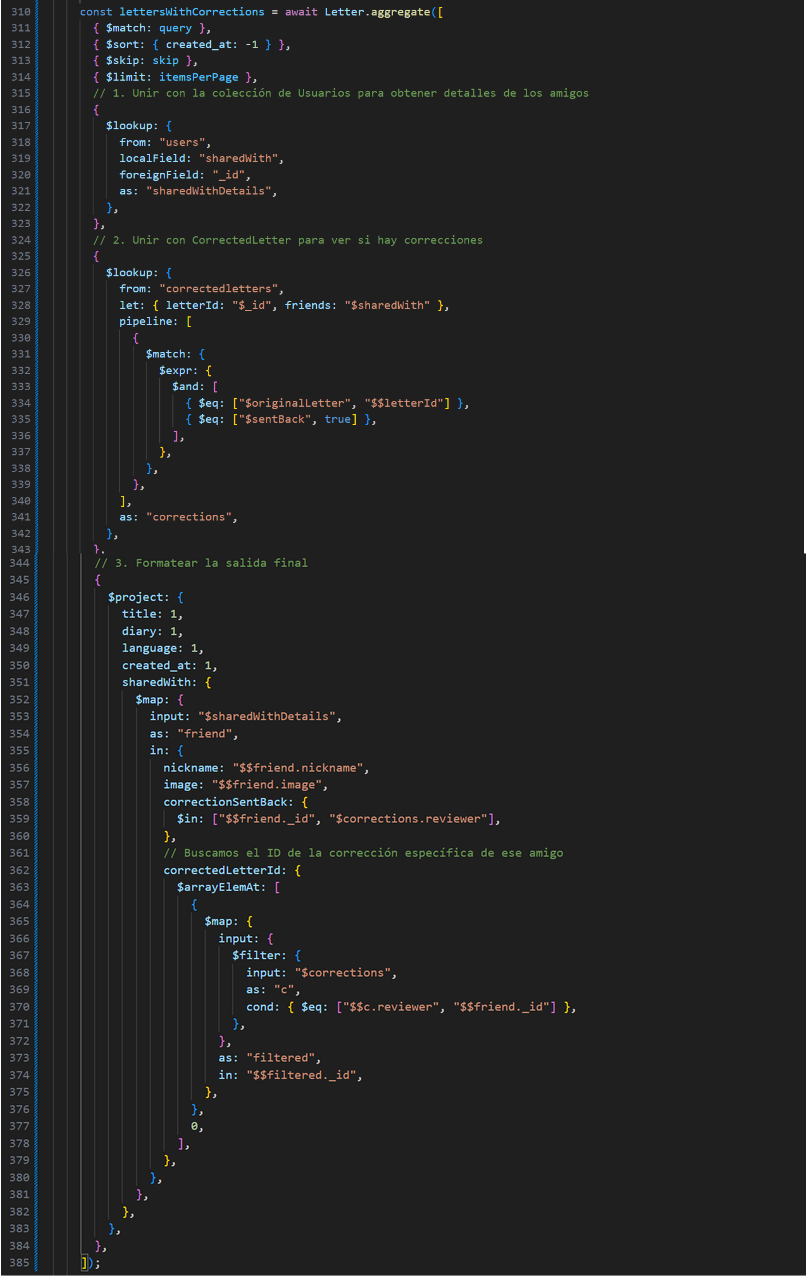
\includegraphics[width=\textwidth]{./imagenes/aggregate3.png}
    \caption{Consulta optimizada 1}
    \label{fig:aggregate}
\end{figure}